This chapter includes the design decision taken while implementing the \acrfull{wdias}, and how is the system got adapted from the systems analyzed in Chapter \ref{ch:literature}. %, then how is it trying to propose a better system with overcoming the issues.
In Section \ref{se:high_level_design} a brief discussion on how the weather forecasting is happening and why it need to interact with multiple data formats is presented. Then following subsections define few termelogy which are using in the \acrshort{wdias}, and scope of the thesis.
Section \ref{se:architectural_decisions} that we evolve over while designing and implementing the \acrshort{wdias}.
The section \ref{se:microservice} gives better understanding of the microservice architectural concepts follows while implementing the \acrshort{wdias}.
Then the reason behind developing Heirarchital Database and technologies use for that discussed in the section \ref{se:db_struct}.
Throw out the section \ref{se:data_preprocess} discussed about how the \acrshort{wdias} enable for data preprocessing and adding capabilities via concept of Extensions.
Finally, in Section \ref{se:query} includes details on how to perform timeseries search and geo based queries.

%%%%%%%%%%%%%%%%%%%%%%%%%%%%%%%%%%%%%%%%%%%%%%%%%%%%%%%%%%%%%%%%%%%%%%%%%%%%%%%%
\section{High-level Design}
\label{se:high_level_design}

To get overall idea on the flow of weather prediction, let us look into one of flows using in \acrshort{curw} \cite{CUrWSL2017SL}.
\dbc{Use CUrW-SL}

\begin{enumerate}
    \item Extract GRIB WRF model data to netCDF
    \item From netCDF to CSV of each location data, then feed to HEC-HMS and get the output as CSV
    \item CSV and Rain cell Grid feed into the FLO2D, and get the water level as Grid ASCII files after completion of simulation
    \item Upload ASCII files to ArcGIS create Raster files, then use for the LOSS Estimation
\end{enumerate}
When looked into the above flow, it clear understanding on multiple data formats using while weather predictions.
Other than that, to correct the model outputs, it required to collect real time data such as;
\begin{itemize}
    \item Automated weather station sending data in higher frequent intervals via HTTP protocol
    \item Automated water level stations send data in higher frequency
\end{itemize}
Other than above there are many data formats using for handling data based on devices and standards which are using. Also, for data modeling, it needs to convert the data into model compatible data format, then after successfully run the model it needs to collect data from the model output data formats.

\subsection{Modules of a Weather Data System}
\label{subse:modules_weather_data_integration_sys}

Figure \ref{fi:wdia_components} shows the basic functions of a Weather data integration and assimilation system which consists of the following modules:
\begin{figure}[htbp]
\centerline{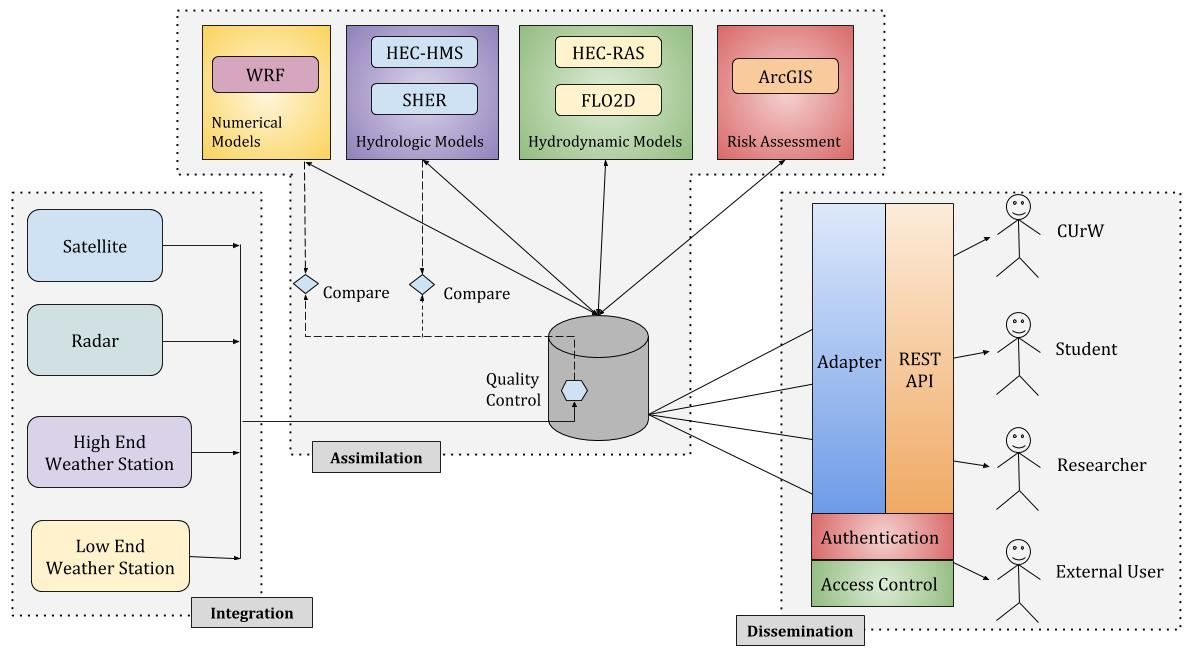
\includegraphics[width=0.8\textwidth]{method/misc/weather_data_system_components.jpg}}
\caption{Modules of a weather data system.}
\label{fi:wdia_components}
\end{figure}

\paragraph{Integration}-- The system should capable of integrating data from different source such as satellite data, high end and low end weather station etc. And the system should be able to handle multidimensional spatial and temporal weather data efficiently and optimally. 
\subsubsection{Assimilation}
Then the system should be able to fulfill weather models varying data requirements. Also those models reproduce large set of redundant data, thus system should store the bulk data while optimizing the disk space.
\paragraph{Dissemination}-- Then different users should be able to retrieve data as they required. Also the users should be able to easy to search into the available that in the system base on timeseries metadata or based on Geo queries.

\paragraph{Timeseries}-- A timeseries is simply a series of data points ordered in time. In weather domain, it interest in timeseries in perspective of observations to forecasting. Each timeseries, the data points can be form in different formats as well. For example, scalar (0D), vector (1D), grid (2D), and polygon (2D).
dbc{Why are you referring to timeseries here? It's not one of the 3 key components in Fig. 3.1.}

In the proof of concept design described below, WDIAS focuses on handling scalar, vector and grid timeseries data. However, the system could be extended to handle polygon-based timeseries as well.

\subsubsection{Base of WDIAS architecture}
\dbc{What's Base of WDIAS architecture?}
\hl{The base of WDIAS architecture origins based on attributes of a timeseries.} %There are many attributes to differentiate timeseries one from another. But 
Among many attribute to differentiate a timeseries from another, the following can be consider as the key attributes in uniquely identify a timeseries from another: % for the \acrshort{wdias}.
\dbc{Highlighted sentence doesn't make sense to me. All yellow highlights mean they are not clear.}

\begin{itemize}
    \item Module -- module that generates the timeseries
    \item Value type -- Scalar, vector, grid, or polygon
    \item Location of readings
    \item Parameter -- measuared parameter
    \item hl{Timeseries type}
    \begin{itemize}
        \item Sources -- External or simulated
        \item Category -- Historical or forecast
    \end{itemize}
    \item Time step
\end{itemize}
\dbc{Use bullets only when essential. Other places use paragraphs.}

A detail description of the above attributes are presented in Section \ref{se:db_struct}.